\chapter{Migration von Sormas}
\todo{sich's aus dem text verbannen}

\section{SORMAS}
\label{ref:sormas_strucure}
Um die Anwendung \ac{SORMAS-ÖGD}(im weiteren zur Vereinfachung nur noch \ac{SORMAS}) erfolgreich migrieren zu können, müssen wir diese zunächst in ihre einzelnen Teile runterbrechen und identifizierne wofür die einzelnen Komponenten verantwortlich sind.
Da \ac{SORMAS} zum aktuellen Zeitpunkt als containerisierte Anwendung ausgerollt wird kann sich hier an der \textit{docker-compose.yaml}\footnote{https://github.com/hzi-braunschweig/SORMAS-Docker/blob/master/docker-compose.yml} orientiert werden.
Diese beschriebt 5 Container, die zusammen die Anwendung bilden.
\begin{itemize}
    \item sormas-application \\ Der Payara-Server auf dem die \ac{SORMAS}-Applikation gehostet wird.
    \item sormas-postgres \\ Die Datenbank in der die Daten aus der Anwendung gespeichert werden.
    \item sormas-pg-dump \\ Dieser Container ist ausschließlich dafür verantwortlich in bestimmten Zeitabständen einen Datenbankdump der Postgres-Datenbank zu machen.
    \item sormas-apache2 \\ Der Webserver ist für die Terminierung der \ac{SSL}-Zertifikate verantwortlich
    \item autoheal \\ Damit können gestoppte oder ungesunde Container neu gestartet werden
\end{itemize}
Da die Anwendung nach Kubernetes migriert werden soll, können einige der Funktionen von den Kubernetes-eigenen Funktionalitäten übernommen werden. 
Der Ingress kann die Terminierung der \ac{SSL} Zertifikate managen und wird den Apache Webserver ersetzen.
Die Autoheal Funktion gehört zu den Grundfunktionen von Kubernetes und muss nicht extra implementiert werden, wenn die Anwendung als ReplicaSet oder Deployment ausgerollt wird.
Der Container, der nur die Datenbank Dumps ausführt, kann durch einen Cronjob abgebildet werden. 
Die einzigen Container die dann noch übernommen werden sind der Payara-Server und die PostgreSQL-Datenbank.
Zusätzlich müssen Ingress und Cronjob konfiguriert werden. \\
Doch zunächst sollen einzelne Funktionen von Kata getestet werden.


\section{Erste Tests mit der Kata Runtime}
Noch bevor begonnen wurde das Cluster aufzubauen, wurden erste Test mit der Kata-Runtime durchgeführt. 
Mit diesen wurde überprüft ob schon im voraus Probleme identifiziert werden konnten, die die Umsetzung verhindern würden. 

\subsection{Docker Kata Integration}
Als erstes wurde ein Container in der Kata Runtime über die bereits installiert Container Engine Docker gestartet.
Mit dem Command \texttt{uname -a} kann der in dem Container verwendete Kernel ausgegeben werden. 
Wenn man diesen mit dem Kernel des Host Systems vergleicht lässt sich feststellen ob beide auf dem gleich Kernel laufen, wie es bei Docker containern der FAll wäre, oder ob ein eigener Kernel für die VM virtualisiert wurde.
\\
Über Docker lassen sich Kata-Container mit der \texttt{--runtime=kata} starten.
Als Images wurden kleine Alpine-Container gewählt.
Um einen Vergleich zwischen beiden Runtimes zeihen zu können wurde ein kurzen Skript gechrieben, dass die Startup-Zeiten in eine Datei schreibt.
Das Skript unter \ref{lst:startuptimes} ergab auf meiner Maschine eine zeitliche Differenz von ca. einer Sekunde wie aus \ref{app:startuptimecomparison} zu entnehmen ist. 
Die wichtigste Erkenntnis an dieser Stelle ist jedoch, dass die Container in der neuen Runtime problemlos starten, und dazu tatsächlich einen anderen Kernel gestartet bekommen.

\begin{lstlisting}[language=bash, caption={compare\_startup\_times.sh}, label=lst:startuptimes]
#!/bin/bash
touch startuptime_comparison
echo runc: > startuptime_comparison
{ time docker run --rm --runtime=runc archlinux sh -c 'uname -r'; } 2>> startuptime_comparison
echo kata-runtime: >> startuptime_comparison
{ time docker run --rm --runtime=kata archlinux sh -c 'uname -r'; } 2>> startuptime_comparison
\end{lstlisting}

\subsection{Webapp in Kata}
\label{ref:kata_plug_and_play}
Im nächsten Test soll das Deployment einer Web-Anwendung in Kata gestestet werden. 
Dafür habe ich das Docker-Image eiener Website zum Thema der Web\ac{API}s verwendet, das während des letzten Semesters erstellt wurde, gewählt. 
Tatsächlich mussten hier gar keine Anpassungen oder Ähnliches vorgenommen werden. 
Die \texttt{runtime}-Flag wurde gesetzt und beim Start konnte der andere Kernel nachgewiesen werden.
Ansonsten ließen sich keine Änderungen in dem Verhalten der Anwendung feststellen. 
Das Austauschen der Runtime verlief komplett nach dem von Kata Angestrebten Plug-and-Play Prinzip.
Hier wurden die Möglichkeiten, die durch das einheitliche Verwenden der Schnittstellen ermöglicht werden, deutlich. 

\subsection{PostgreSQl in Kata}
Als letzter grundlegender Test sollte eine PostgreSQL Anwendung in der Kata-Runtime deployed werden. 
Dabei wurden aufgrund der simplen Migration der Webapp keine größeren Probleme erwartet.
Doch an dieser Stelle machten sich zum ersten Mal Probleme mit der Kata-Runtime bemerkbar.
\\
Das Starten der Anwendung war noch sehr uproblemantisch, alle bnötigten Variablen konnten über eine enviroments-Datei übertragen werden und die Runtime wie zuvor über die entsprechende Flag definiert werden. 
Wurde der Container nach dem Start der Anwendung jedoch betreten und man versucht von dort aus in die Postgres Datenbank zu kommen, erhielt man folgenden Fehler:
\\\texttt{could not connect to server, temporary failure in name resolution}\\
Die Datenbank ist allerdings von außerhalb erreichbar, wurde kein \texttt{docker exec} in den Container ausgeführt, sondern direkt von der Host-Maschine aus der ZUgriff auf die Datenbank gestartet, konnte diese ohne Probleme bedient und gemanaged werden. 
Das Problem ließ sich zwar in der dafür aufgebrachten Zeit nicht lösen, da die Datenbank aber trotzdem erreicht wurden konnte sollte diese Einschränkung kein Problme darstellen. 

Die grundlegenden Tests können damit als abgeschlossen betrachtet werden und es kann mit dem nächsten Schritt, dem Übersetzen der docker-compose Datei zu Kubernetes Manifesten, begonnen werden. 
Zunächst muss dieser Schritt getan werden, damit anschließend die Runtime auf Kata umgestellt und dann gedebugged werden kann. 


\section{Migration der Anwendung nach Kubernetes}
\todo{Umstrukturierung}
\subsection{Struktur}
Als erstes wurde die Struktur der Kubernetes Anwendung geplant. 
Die schon in Absatz \ref{ref:sormas_strucure} festgehalten, können einige Container ignoriert werden, da Ihre Funktion standartmäßig in Kubernetes integriert ist. 
Die restlichen Container müssen jedoch zu Deployments oder StatefulStes übersetzt werden, mit Services zugänglich gemacht, und mit Secrets sowie ConfigMaps konfiguriert. 
Außerdem müssen den Anwendunge \ac{PV}s zugeordnet werden und sie müssen mittels eines Ingresses erreichbar gemacht werden.
Der genaue Aufbau wurde in Abildung \ref{fig:sormas_kubernetes} dargestellt. 
Aus Gründen der Überscihtlichkeit wurde hierbei auf die Darstellung der Backup-Funktionalitäten verzichtet, diese werden später genauer erklärt.

\begin{figure}[h!]
\centering    
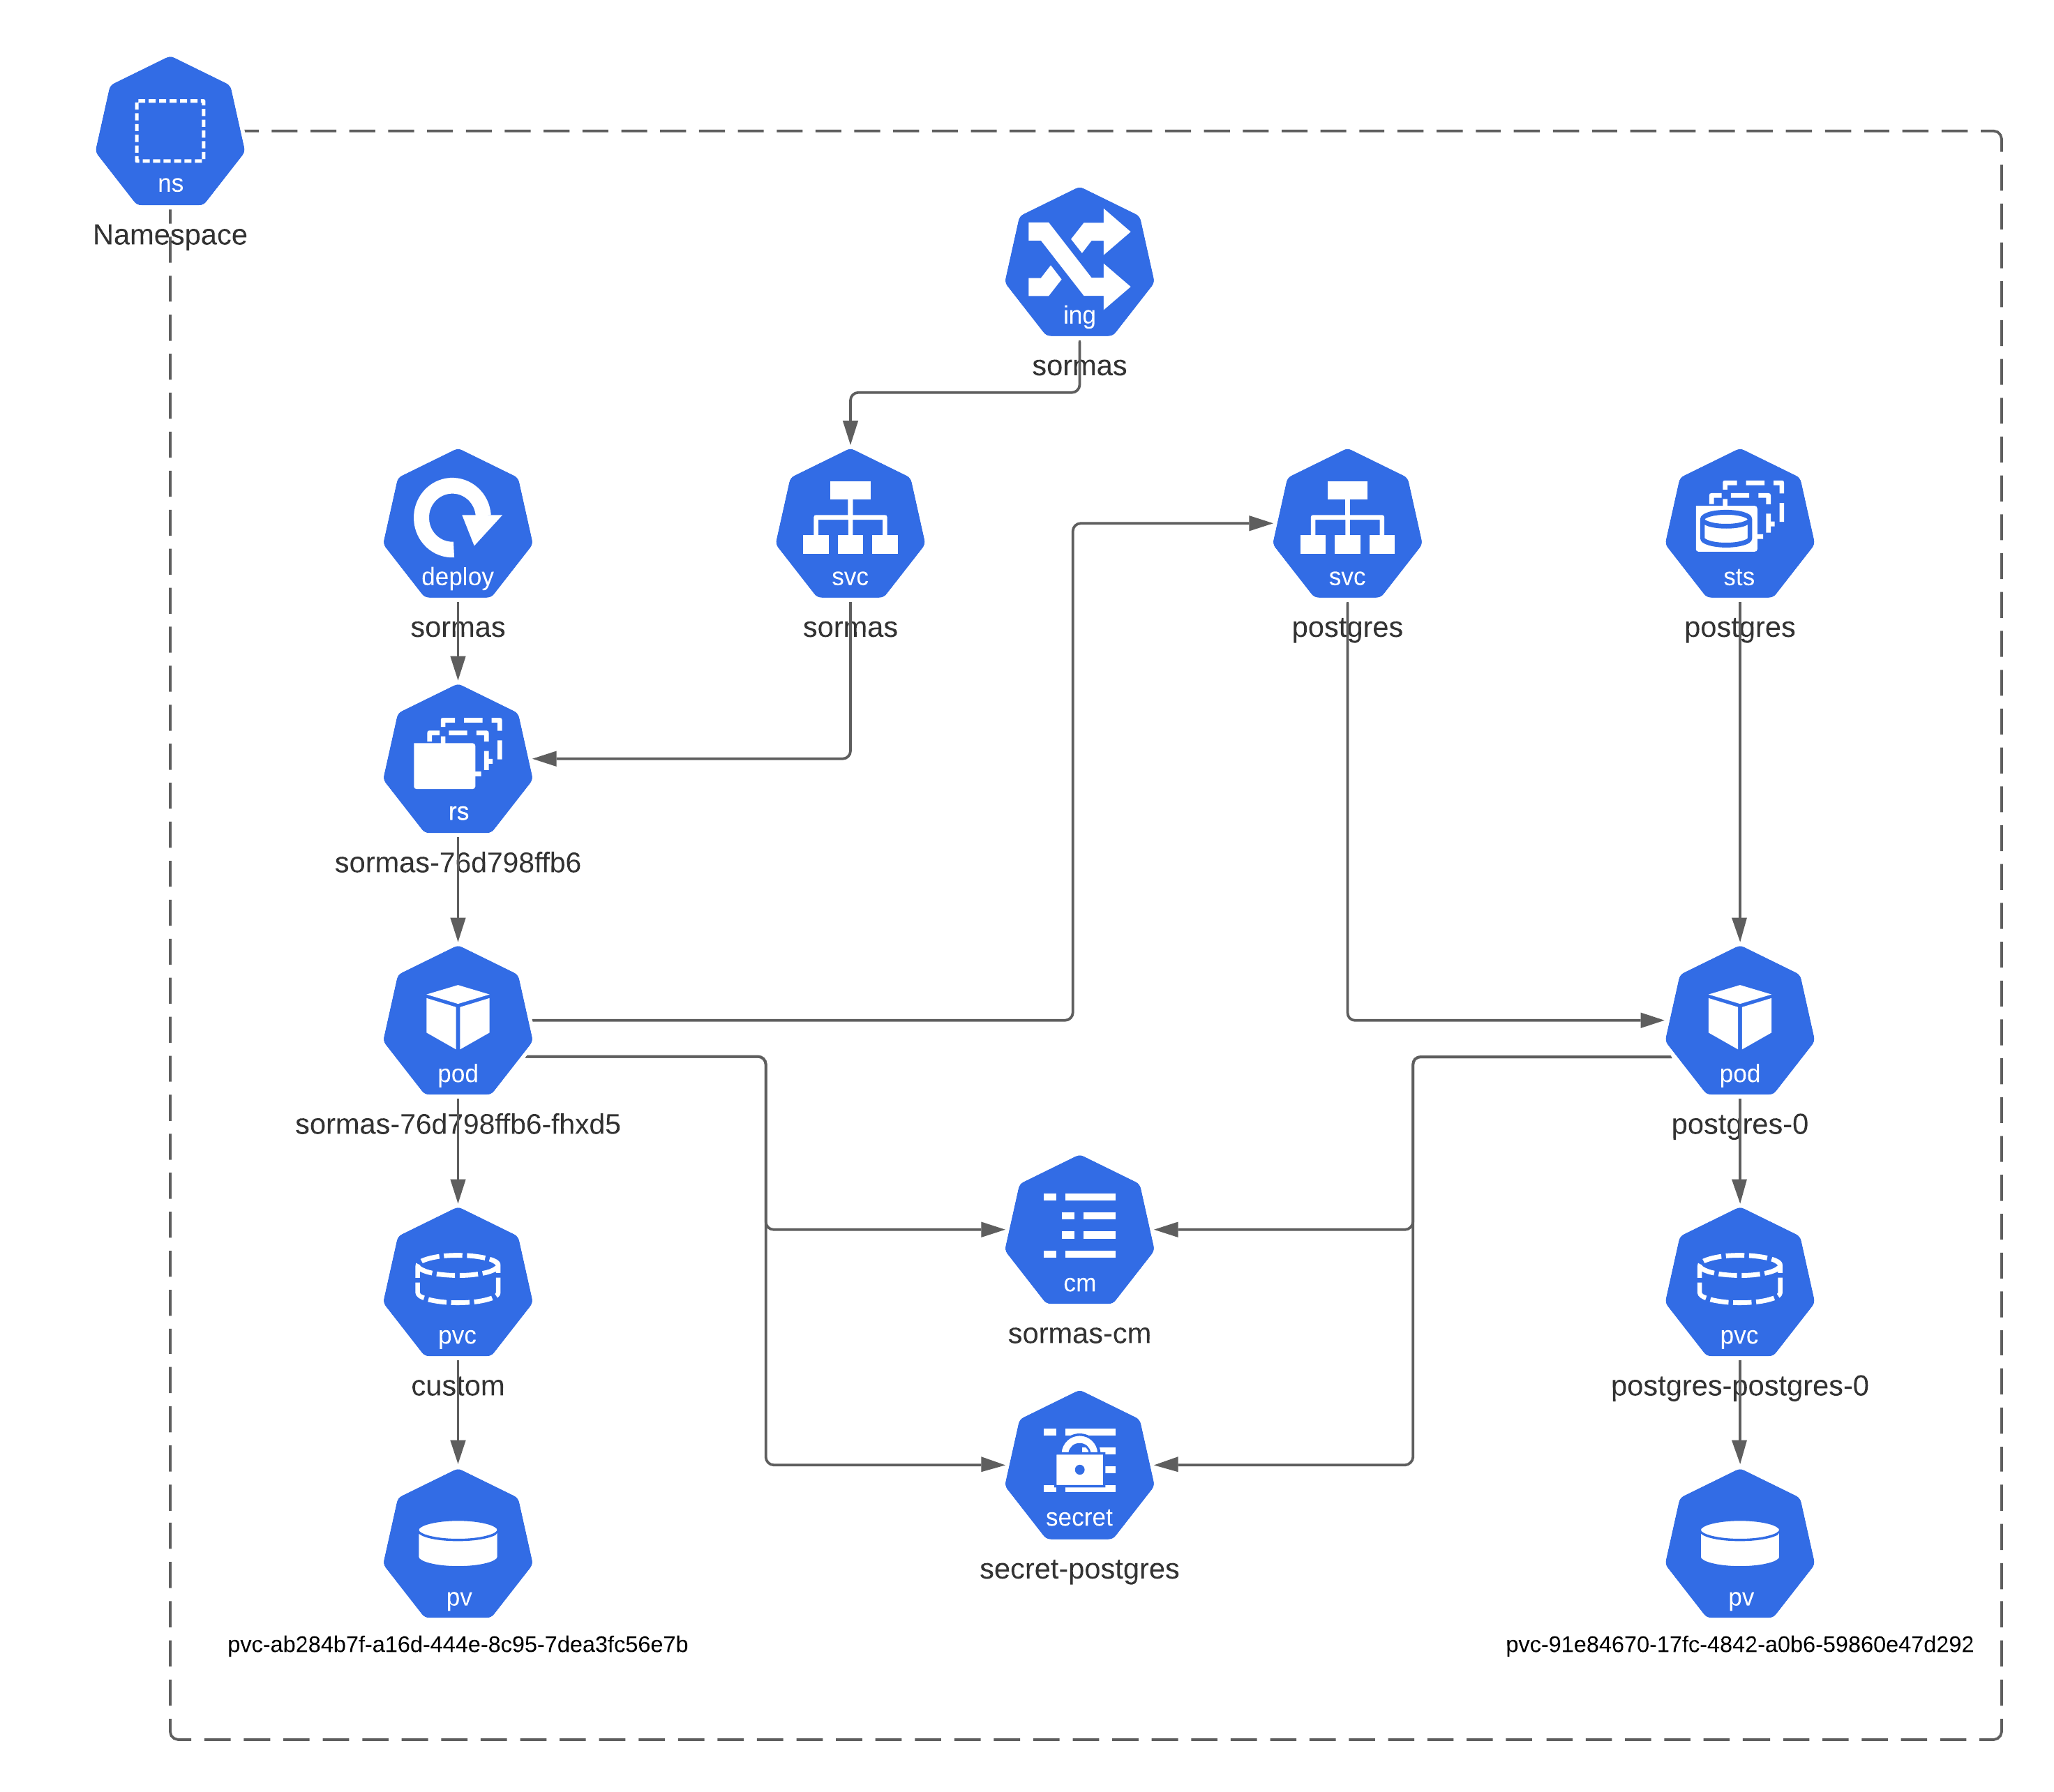
\includegraphics[width=\textwidth]{bilder/sormas_kubernetes.png}
\caption{SORMAS in Kubernetes}
\label{fig:sormas_kubernetes}
\end{figure}

Als Element zur Trennung und Organisation der einzelnen \ac{SORMAS}-Instanzen wird für jedes \ac{GA} ein eigener Namespace angelegt.
So kann jeder Pod genau einem \ac{GA} zugeordnet werden.\\
Wie zuvor angemerkt, ersetzt der Ingress an dieser Stelle den zuvor zur \ac{SSL}-Terminierung benötigten Apache2 Webserver.\\
Die Datenbank wird in einem StatefulSet ausgerollt, da diese durch die genaue Bestimmung der Pods besser persistent gestaltet werden kann.
Das StatefulSet erstellt dann seinen benötigten Pod, der über ein \ac{PVC} sein \ac{PV} zugeordnet bekommt. 
Die Konfiguration des Pods soll ausschließlich in der ConfigMap und dem Secret stattfinden, sodass nur an einer Stelle Anpassungen vorgenommen werden müssen.
Der Pod kann durch das Einrichtigen eins Services für andere Instanzen im selben Namespace erreichbar gemacht werden.\\
Der Payara-Server wird mit einem Deployment-Manifest ausgerollt. 
Die Eigenschaften des StatefulSets werden nicht benötigt und die Vorteile in Hinsicht auf das erleichterte Updaten der Software werden für zu erwartende Updates nützlich sein.
Das Deployment erstellt dann das entsprechende ReplicaSet und dieses den Pod. 
\ac{PV} und Konfiguration werden analog zu Postgres gemanaged. 
Der Service wählt mittels des Selectors allerdings das ReplicaSet und nicht den Pod selbst.


\subsection{Schreiben der Kubernetes Manifeste}

Alle geschriebenen Manifeste, auch die auf die in diesem Abschnitt nicht weiter eingegangen wird, sind auf Github veröffentlicht und können dort unter \url{https://github.com/robbmue/katanetes_sormas/tree/master/manifests} eingesehen werden. 

Beim Schreiben der Manifeste diente die \textit{docker-compose.yml}\footnote{https://github.com/hzi-braunschweig/SORMAS-Docker/blob/master/docker-compose.yml} als Vorlage.
Aus dieser wurden zunächst einmal alle Services eliminiert die in Kubernets nicht weiter benötigt werden, namentlich den Autoheal, den Apache2 Webserver und den pg-dump.
Die beiden letzen Teile der Anwendung wurden dann entsprechend der vorhergehenden Planung in jeweils ein Deployment und ein StatefulSet übersetzt.
Zuerst wurde ein Namespace für die komplette Anwendung angelegt, in dem alle restlichen Teile deployed werden.

\hfill \newline
\subsubsection{Payara Deployment}
Bei dem Payara Server ist vor allem wichtig, deren speziellen Port in das Manifest miteinzubinden.
Payara nutzt als Standart-Port 6080 und als Admin-Port 6048, diese werden unter den Namen \texttt{payara} und \texttt{payara-admin} dem Deployment hinzugefügt.
Abhängig von diesen ist auch die liveness- und readinessProbe, hier werden diese mit einem \ac{HTTP}-GET auf den entsprechenden Port und den \ac{SORMAS}-Pfad \texttt{/sormas-ui/login} realisiert.
Wenn diese Seite erreichbar ist, kann von einer funktionierenden Instanz ausgegangen werden.
Der Service, der auf diese Anwendung verweist, wird so konfiguriert, dass dieser auf Port 80 lauscht aber alle eingehenden Anfragen an Port 6080 des Payara-Pods weiterleitet.
So kann der ungewöhnliche Port des Payara-Servers in einen Standart-Port umgewandelt werden. 
Der Ingress wiederum zeigt auf den Service und Sorgt dafür, dass die Anwendung von außerhalb erreichbar ist.

Des weiteren muss das \ac{PV} mittels des \ac{PVC} eingebunden werden und die Enviroment-Variablen müssen gesetzt werden. 
Der \ac{PVC} wird unter dem Punkt \texttt{volumes} dem Pod zugewiesen und unter \texttt{volumeMounts} wird der Pfad angegeben, an der das Volume eingahngen werden soll. 
Die Variablen setzt man unter dem Punkt \texttt{env}, hier kann sowohl auf ein Secret, als auch auf eine ConfigMap zugegriffen werden und diese zu setzen.
Es könnten auch direkt in dem Deployment die korrekten Werte gesetzt werden, mit der ConfigMap und dem Secret wird jedoch erreicht, dass Änderungen nur an möglichst wenigen Stellen vorgenommen werden müssen.
Außerdem wird auch das StatefulSet auf die gleichen Dateien zugreifen, und so kann garantiert werden, dass beide Anwendungen übereinstimmende Werte geliefert bekommen.

Zuletzt werden noch Limits für \ac{CPU} und Memory-Nutzung gesetzt. 

Auf die Manifeste für den \ac{PVC}, die ConfigMap und das Secret soll hier nicht weiter eingegangen werden da diese keine Großen Besonderheiten enthalten. 

\hfill \newline
\subsubsection{SORMAS StatefulSet}
Für die Datenbank wurden Konfigurationen analog zu denen des Payara-Servers vorgenommen.
Der Port 5432 wurde freigegeben, die Enviroment Variablen und der \ac{PVC} wurden eingebunden sowie limits gesetzt.
Eine Besonderheit in diesem Manifest ist, dass mit dem \texttt{args} Parameter gearbeitet werden muss. 
Es muss eine Änderung an dem Parameter \texttt{max\_prepared\_connections} in der \textit{postgresql.conf} vorgenommen werden, damit \ac{SORMAS} starten kann. 
Der Postgres Container startet immer mit dem \texttt{psql} Kommando, also kann mittels des Arguments \texttt{-c config\_file=/etc/postgresql/postgresql.conf} die Config eingelesen werden.

Auf den Service und den \ac{PVC} soll an dieser Stelle nicht weiter eingegangen werden, sie können auf Github nachgelesen werden. 


\hfill \newline
\subsubsection{Backup}
Als Backup-Lösung wurde Stash\footnote{https://stash.run/\#} von AppsCode\footnote{https://appscode.com/} gewählt.
Die Software erlaubt es unter anderem Backups auf einem lokalen Storage zu erstellen und mit Datenbankdumps zu arbeiten, nicht nur mit Volume Snapshots.

Bei Netzlink wird ein lokaler Minio\footnote{https://min.io/} \ac{S3}-Storage gehostet, in dem die Backups gespeichert werden können.
Damit Stash die Verbindung zu diesem aufbauen kann muss zunächst ein Secret erstellt werden, dass die Anmeldedaten für den \ac{S3} Storage beinhaltet.
Aufbauend darauf kann dann die \ac{CRD} \texttt{Repository} deployed werden. 
Diese gibt die Addresse des \ac{S3} Storages an, sowie den Bucket in den gespeichert werden soll und das zur Organisation verwendete Prefix.
Außerdem beinhaltet die Repository-Ressource auch das zuvor definierte Secret und bindet dieses so an das Repository.
\\
Als nächstes wird die \ac{CRD} \texttt{AppBinding} erstellt. 
Über dieses AppBinding wird benötigt um auf die Datenbank zuzugreifen. 
Dazu braucht es den Service und Port, sowie das Schema und den Typen der Datenbank und letzten endes ein Secret, aus dem der Datenbanknutzer und sein Password ausgelesen werden können.
In dieser einen \ac{CRD} sind dann also alle Informationen gesammelt um auf die Datenbank zuzugreifen und in dem Repository ist definiert wohin das Backup gespeichert werden soll.
Als letztes fehlt also nur noch eine Ressource, die das Backup anstößt.
\\
Diese \ac{CRD} nennt sich \texttt{BackupConfiguration}. 
In ihr wird 
\begin{itemize}
    \item das \texttt{AppBinding} und das \texttt{Repository} zusammengetragen
    \item der auszuführende Task angegeben (in dem Version und Art der Datenbank festgelegt sind)
    \item eine \texttt{retentionPolicy} definiert (diese gibt an wie viele der erstellten Backups erhalten bleiben sollen)
    \item der \texttt{schedule} in CronJob Syntax angegeben
\end{itemize}
Stash erzeugt aus diesen \ac{CRD}s dann Ressourcen, mit denen Kubernetes arbeiten kann.
Alle benötigten Informationen werden in einem Kubernetes nativen CronJob zusammengetragen.
Ein CronJob in Kubernets erstellt sich immer zur definierten Zeit einen Job. 
Ein Job wiederum erstellt einen oder mehrere Container, die nur eine genau abgegrenzte Aufgabe haben, und stellt sicher dass diese erfolgreich terminieren. 
In diesem Fall ist die Aufgabe das Erstellen das Datenbankdumps, das Verschlüsseln und Kopieren der verschlüsselten Daten auf den \ac{S3} Storage plus das Löschen der überschüssigen, bereits vorhandenen Datenbankdumps.
Nach der erfolgreichen Ausführung all dieser Operationen terminiert der Job und alle Pods werden gestoppt. 
So kann garantiert werden, dass das Backup nur während der Ausführung Compute-Ressourcen verbraucht. 

Wird nun eine \ac{SORMAS}-Instanz mit diesen Manifesten deployed ist die komplette Funktionalität der urspürunglichen Anwendung abgebildet.

\subsubsection{Tests}
\label{ref:tests}
Als erstes wurde kontrolliert, ob der Payara Server erreichbar ist.
Dazu muss ein Host-Eintrag auf dem Localhost gesetzt werden, da das Test Cluster nicht in der \ac{DMZ} aufgebaut wurde, keinen \ac{DNS} Eintrag hat und nur als dem Netzlink Netzwerk zu erreichen ist. 
Wenn der Payara-Server erreichbar ist, wird als nächstes überprüft, ob das \ac{SORMAS}-\ac{GUI} erreichbar ist.
Auf der \ac{GUI} kann dann gechecked werden, ob mit den konfigurierten Usern eine Anmeldung durchgeführt werden kann und somit der Login Prozess funktioniert.
Nachdem sich angemeldet wurde, werden einige Fälle eingetragen, bearbeitet und gelöscht um die Funktionalität der Anwendung sowie die Postgres Integration zu prüfen.

Um die Autoheal Funktion zu testen, kann einfach der Sormas Pod gelöscht und dann die Erstellung des neuen Pods abbgewartet werden.
Wenn dieser von dem ReplicaSet wieder gebaut wird, ist die Autoheal Funktion korrekt abgebildet.

Zuletzt wird die BackUp Funktion überprüft.
Dazu werden einige Einträge in der Datenbank vorgenommen, und ein BackUp-Job angestoßen. 
Nachdem dieser durchgelaufen ist werden die Daten aus der PostgreSQL-Datenbank gelöscht.
Über einen Restore-Job wird versucht die zuvor gelöschten Daten aus den Datenbankdump wiederherzustellen. 
Wenn der Restore-Job erfolgreich beendet wird und die Daten wieder in der Anwendung auftauchen, ist die Backupfunktionalität positiv getestet.


\section{Migration der Anwendung zur Kata-Runtime}
Theoretisch funktioniert die Migratio der Anwendung nach dem gleichen Plug-and-Play Prinzip wie bereits in Abschnitt \ref{ref:kata_plug_and_play} beschrieben.
Die Runtime ist für Containerd bereits in Abschnitt \ref{ref:kata_config} als Plugin definiert und muss nur als Parameter in die Manifeste eingepflegt werden.
Der Parameter wird wie im Quelltext \ref{lst:runtimeClassName} gesetzt.
Leider ließ sich dieses Verfahren jedoch in der Praxis nicht so problemlos umsetzen, die Probleme und Lösungen sollen in den nächsten Absätzen aufgezeigt werden. 

\begin{lstlisting}[language=yaml, caption=runtimeClassName, label=lst:runtimeClassName]
apiVersion: apps/v1
kind: Deployment
metadata:
  name: sormas
  namespace: ga-test
spec: 
  replicas: 1
  selector: 
    matchLabels:
      run: sormas
  template:
    metadata:
      labels:
        run: sormas
    spec:
      runtimeClassName: kata
      containers:
        - image: hzibraunschweig/sormas-application
          name: sormas
...
\end{lstlisting}


\subsection{Migration des Payara Servers}
Der Payara Server wurde als erstes zur Migration ausgewählt. 
Der Parameter wurde entsprechend gesetzt und die komplette Anwendung wurde ausgerollt. 

Zuerst schien es als würde die Anwendung auf dem Payara-Server gar nicht starten. 
Der Payara Server selbst war zwar erreichbar, doch die Anwendung darauf war nicht erreichbar.
Beim genaueren Beobachten des Server konnte festgestellt werden, dass die \ac{SORMAS}-\ac{GUI} für einige Sekunden erreichbar ist und man sich sogar anmelden kann, bis diese aus irgendeinem Grund wieder verschwandt.
In den Logs wurden tausende Zeilen Java Stack Traces ausgegeben. \todo{Stack traces nachstellen. Recherche auf Home-Laptop! History ca. Anfang September}
Die Analyse der Logs ergab, dass die Anwendung zu einem bestimmten Zeitpunkt \texttt{succsessfully autodeployed} wurde, der Payara-Server aber nicht wie unter runc an dieser Stelle den Deployment Process beendete sondern wieder damit begann die Annwendung zu deployen.
Als diese Erkenntnis gewonnen war, wurde untersucht welche Dateien zu welchen Zeitpunkten im Filesystem erstellt wurden und wie sich diese von dem Deployment-Prozess in runc unterscheiden. 
Es ließ sich jedoch keine Abweichung während des Deployment Prozesses feststellen.
Auch nach langer intensiver Recherche und Troubleshooting mit qualifizierten Kollegen konnte kein Grund dafür gefunden werden, dass der Autodeployment-Prozess nicht nach dem erfolgreichen Ausrollen der Anwendung stoppt. 
\\
Das Autodeployment Feature von Payara muss also für unseren Use-Case umgangen werden. 
Dazu wurden die offiziellen Dockerfiles der \ac{SORMAS}-Applikation\footnote{https://github.com/hzi-braunschweig/SORMAS-Docker/tree/master/sormas} untersucht. 
In diesem werden die Skripte \textit{setup-server.sh} und \textit{start-server.sh} genutzt.
In dem \textit{start-server.sh} Skript zum Deployen der Anwendung als letztes alle \textit{.ear} und \textit{.war} Dateien in den Autodeployment Ordner kopiert.
Wird dann der Payara Server mittels \texttt{asadmin start-domain} gestartet versucht der Server alle Datein in dem Autodeployment Ordner auszurollen.
Um zu verhindern, dass der Autodeploy-Prozess die Anwendung immer wieder zerschießt, muss Sie auf einem anderen Weg ausgerollt werden.
Dazu wurde das \textit{start-server.sh} Skript entsprechend angepasst, sodass die einzelnen \textit{.ear} und \textit{.war} Dateien mittels des \texttt{asadmin deploy} Kommandos ausgerollt werden.
Mit diesen Änderungen wird die Autodeploy-Funktion komplett ausgesetzt, sodass die Anwendung nun nicht mehr vom Payara-Server selbst abgeschossen werden sollte.
Es wurde ein neues Container-Image mit diesen Anpassungen erstellt und auf der Docker-Registry\footnote{https://hub.docker.com/repository/docker/robbmue/sormas\_kata} veröffentlicht, damit Kubernetes sich dieses Image ziehen kann.
Nachdem das neue Image in die Manifeste eingebunden, und die Anwendung neu ausgerollt wurde, konnte mit den zuvor unter Abschnitt \ref{ref:tests} beschrieben Tests gezeigt werden, dass der \ac{SORMAS}-Payara nun unter Kata voll funktionsfähig war.


\subsection{Migration der PostgreSQl-Datenbank}
Als nächster und letzter Teil der Anwendung muss nun noch die Datenbank mit ihrem eigenen Kernel versehen werden.
Dazu wurde zuerst wieder der benötigte Parameter in dem StatefulSet Manifest gesetzt und anschließend die Anwendung ausgerollt.

\todo{Problmestellung auf Laptop recherchieren, ungefähr 10.9.}

Nach ausführlichen Tests mit dem Image des HZI ließen sich die Netzwerk-Probleme noch immer nicht beheben.
Um die Probleme zu verstehen wurde mit allen möglichen Postgres-Images experimentiert.
Nach einigen Tests ließ sich feststellen, dass die Probleme ausschließlich in den Alpine-Versionen der Postgres Images auftreten, aber nicht in den Postgres Images auf Debian Basis. 
Die Herausforderung besteht also darin, das Image des \ac{HZI}, das auf dem Postgres-Image auf Alpine Basis aufbaut, in einem neuen Image abzubilden, das auf dem Postgres-Debian image basiert.
Die Alpine Version wurde vermutlich gewählt um den Container an sich möglichst klein zu halten. 
In \ref{lst:alpine_postgres_size} wird die Größe des Images ermittelt.
Diese beträgt \texttt{450MB}.

\begin{lstlisting}[language=bash, caption={Größe des Postgres Images}, label=lst:alpine_postgres_size]
$  ~ docker images | awk 'NR==1 || /^hzibraunschweig\/sormas-postgres/ {printf "%-33s %-10s %s\n", $1, $2, $NF}'
REPOSITORY                        TAG        SIZE
hzibraunschweig/sormas-postgres   2.8.0      450MB
\end{lstlisting}

Die Untersuchung des Images ergab, dass sehr viele Pakete installiert werden müssen um das Modul \texttt{temporal\_tables} für Postgres zu installieren.
Die folgenden Pakete werden benötigt um das Modul zu installieren und compilieren:
\begin{itemize}
  \item postgresql-server-dev-10
  \item pgxnclient 
  \item make
  \item gcc
\end{itemize}

Nach der Installation des Modules werden sie jedoch nicht mehr benötigt und können deswegen mittel des \texttt{apt}-Feature \texttt{autoremove} wieder entfernt werden. 
So wird versucht das Image trotz der größeren Basis klein zu halten.
Eine Überprüfung der Image-Größe nach dem Bauen ergab, dass das Image durch die Anpassungen sogar kleiner geworden ist und nun nur noch \texttt{373MB} beträgt, wie \ref{lst:debian_postgres_size} zeigt.

\begin{lstlisting}[language=bash, caption={Größe des Debian Images}, label=lst:debian_postgres_size]
$  ~ docker images | awk 'NR==1 || /^robbmue\/postgres_kata/ {printf "%-33s %-10s %s\n", $1, $2, $NF}'
REPOSITORY                        TAG        SIZE
robbmue/postgres_kata             latest     373MB
\end{lstlisting}

Es wurde ein neues Container-Image mit diesen Anpassungen erstellt und auf der Docker-Registry\footnote{https://hub.docker.com/repository/docker/robbmue/postgres\_kata} veröffentlicht, damit Kubernetes sich dieses Image ziehen kann.
Nachdem das neue Image in die Manifeste eingebunden, und die Anwendung neu ausgerollt wurde, konnte mit den zuvor unter Abschnitt \ref{ref:tests} beschrieben Tests gezeigt werden, dass die Postgres-Datenabnk nun unter Kata voll funktionsfähig war.

Das neue Postgres-Dockerfile ist dem Anhang unter \ref{app:small_postgres} zu entnehmen.


\section{Helm Templating}
Im letzten Schritt soll das Deployment nun soweit vereinfacht werden, dass das Bereitstellen einer kompletten Instanz über einen einzigen Befehl durchgeführt werden kann.
Dazu wird \texttt{helm} eingesetzt. 
Die Software bietet vielfältige Möglichkeiten, von denen für dieses Projekt jedoch nur die Templating-Funktion genutzt wird.
Für jedes \ac{GA} soll ein eigener Namespace erstellt werden, zuerst wird also die Namespace Ressoruce getemplated.
Für den Namespace wird der Release-Name verwendet, sodass dafür nichtmal die \textit{values.yaml} angepasst werden muss, in der alle anderen Variablen für das Templating gesetzt werden. 
Der Release-Name wird direkt in dem \texttt{helm install} Befehl mit angegeben, die Syntax ist unter \ref{lst:helm_install} beschrieben, in dem Beispiel wäre das "beispielgesundheitsamt".
Im Anhang unter \ref{app:namespace_template} wird gezeigt wie mit dem Release Name gearbeitet wird. 
Analog dazu werden die Namespaces aller anderen Ressourcen definiert. 

\begin{lstlisting}[language=bash, caption={Syntax des \texttt{helm install} Kommanods}, label=lst:helm_install]
helm install <beispielgesundheitsamt> ./sormas
\end{lstlisting}

Alle anderen Variablen werden über die \textit{values.yaml} gesetzt.
In dieser kann mit Objekten gearbeitet werden, für dieses Projekt gibt es beispielsweise ein Objekt \texttt{image} das die Objekte \texttt{sormas} und \texttt{postgres} enthält, in denen dann Name und Version des Images definiert wird. 
Dieses Beispiel ist dem Anhang unter \ref{app:values_yaml} beigefügt.
Auf diese Werte wird ähnlich wie auf den Release-Name zugegriffen, nur dass der Release durch Values ersetzt wird.
Auf den Sormas Image Namen mit Version wird exempli causa folgenderweise zugegriffen: \texttt{ \{\{ .Values.image.sormas.name \}\}:\{\{ .Values.image.sormas.version\}\} }

Helm bietet auch die Option, Werte die aus der Values Datei eingelesen werden in Pipelines zu senden um sie in irgendeiner Art zu transformieren. 
Diese Funktionalität ermöglicht es, die Werte für die Secrets im Klartext in die Values zu schreiben, um sie dann über eine Pipeline zu verschlüsseln, wie unter \ref{app:secret_template} demonstriert.
Pipelines werden außerdem für das erstellen der ConfigMap Template genutzt. 
An dieser Stelle wird vor allem die \texttt{quote} Funktion verwendet, damit beim Bearbeiten der Values nicht darauf geachtet werden muss, alle Ints zu Strings umzuwandeln. 
Nötig ist das, da ConfigMaps ausschließlich mit Strings arbeiten können.
Für die ConfigMap wird außerdem die \texttt{default} Funktion verwendet, um für Werte die nicht zwingend gesetzt werden müssen einen leeren String einzusetzten falls sie nicht überschrieben werden.
Das Ergebnis ist dem Anhang unter \ref{app:configmap_template} beigefügt.